\documentclass[12pt,a4paper]{article}
\usepackage{graphicx}
\usepackage{amsmath, amssymb}
\usepackage{siunitx}
\usepackage{geometry}
\geometry{margin=2.5cm}
\usepackage{wrapfig}
\usepackage{caption}
\usepackage{subcaption}

\captionsetup[figure]{width=0.8\textwidth}  % for all figures

\begin{document}
\title{Plumbus creation through the use of 3D scanning, FDM printing and
laser-cutting}

\author{
  BSc-5 \\[1em]
  Adam Gabor Bacso \\
  Borys Maksymilian Bobrowski \\
  Greta Klara Wodala \\
  Juan Ruiz \\
  Nikola Dragomirov Dimitrov \\
  Rui Emanuel Vasquez Pacheco
}

\date{October, 2025}
\maketitle
\tableofcontents
\newpage

\section{Introduction}

The goal of the project was to create a 3D printed plumbus -- a fictional
household item from the Rick and Morty universe -- by 3D scanning at least 5
common, physical objects. The scanned files needed to be fabricated using a
Fused Deposition Modeling (FDM) printer along with a base for the object by the
method of laser-cutting.

A plumbus has 5 distinct parts for which 5 real world items have been selected:

\begin{figure}[h]
  \begin{center}
    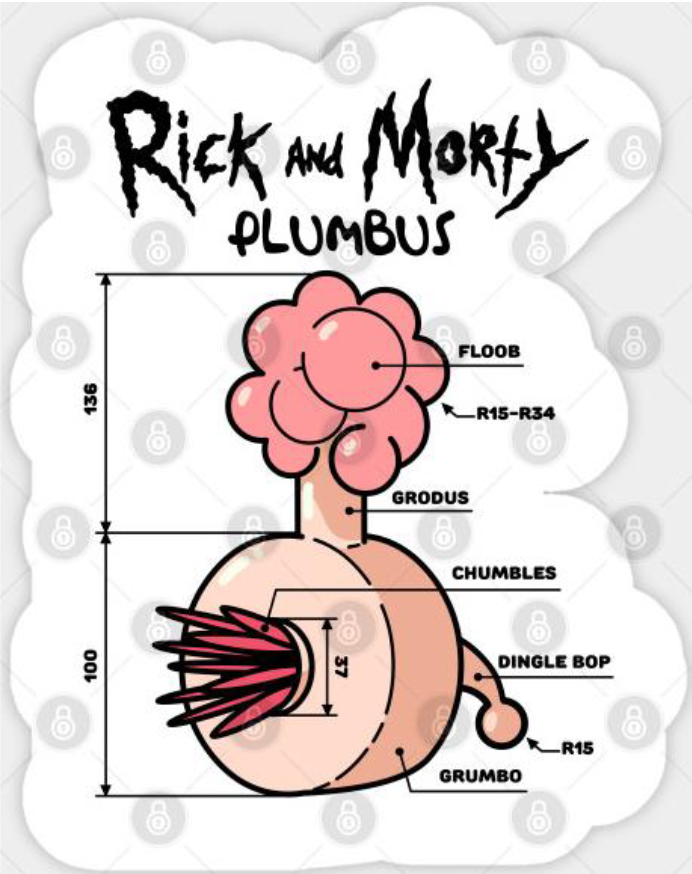
\includegraphics[width=0.4\linewidth]{media/plumbus_drawing.png}
  \end{center}
  \caption{Labeled image of a plumbus with rough dimensions.}
\end{figure}

\begin{itemize}
  \item Floob $\to$ microfiber cloth ball
  \item Grodus $\to$ toilet paper roll core
  \item Chumbles $\to$ brush bristles
  \item Dingle bop $\to$ microfiber cloth cone
  \item Grumbo $\to$ toilet paper roll
\end{itemize}

Objects were chosen from common cleaning supplies to reflect some of the uses of
the plumbus.

\section{Scanning}

The first step in creating the plumbus was to acquire the geometries of the
selected objects.

First, the objects had to be prepared to fit the exact needs of the project. For
some, such as the paper tube, it meant creating additional, more detail-rich
texture while for others it meant modifying their shape and adding a mounting
option to allow scanning on all sides. Most of these modifications were made
with the use of rubber bands.

The first method of 3D scanning was to attempt photogrammetry
with mobile devices. The main issue encountered was the impossibly long upload a
processing times of the apps\footnote{Apps attempted were Polycam, Modelar and
CamToPlan.} that we tried. Blaming the server-based processing, the use of
\emph{Meshroom} was attempted for stitching individual images into a 3D scene,
but it also abandoned due to its extreme hardware and storage requirements.

Finally, a decision has been made to use specialized scanning hardware.
The scanner used was the \emph{EINSTAR VEGA hand scanner},
provided by our professor. With its display and on-device processing, it proved
to be fairly user-friendly, but several issues also presented themselves.

\begin{figure}[h]
  \centering
  \includegraphics[width=0.3\textwidth]{media/scanning.png}
  \caption{The UI of the EINSTAR VEGA gave valuable information such as the
    optimal distance to the scanned object as well as areas that still need more
  definition.}
\end{figure}

\renewcommand{\arraystretch}{2}
\begin{table}[h]

  \centering
  \begin{tabular}{ | p{0.35\linewidth} | p{0.6\linewidth} | }
    \hline
    Issue & Solution \\
    \hline
    Scans would not initiate / not recognize an object's presence. & Starting
    scans from the pedestal used (chair) and only after initialization moving up
    to the desired object. \\
    When scanning the hanging ball, the chair leg obstructed the view to the
    object. & Switching to a detailed scan reduced the working distance.\\
    Some objects, mainly those of paper, lost tracking easily. & Adding dots on
    the exteriors seemed to facilitate tracking by adding distinct features for
    texture based tracking.\\
    \hline
  \end{tabular}
  \caption{List of issues faced with the actions taken to tackle the problem.}
\end{table}

\subsection{Scan cleanup}

The 3D scanner provided the models in STL format. Although the slicer program
used, which would turn the model into machine instructions for the 3D printer,
would accept the format, the scans also included features of the objects'
surroundings. To remove those and to place the individual parts in their final
positions in respect to the whole, each scanned object was imported into
Blender. Blender is a free and open-source 3D computer graphics software tool
with a few clear advantages over traditional computer aided design (CAD)
software which served the project's needs well:

\begin{itemize}
  \item It features an advanced polygonal modeling system, allowing for easy
    vertex manipulation. The meshes generated by the scanner also consist of
    polygons.
  \item The sculpting tool in Blender allows for more refined adjustment of
    organic features.
  \item Although simplistic, there exists a dimensioning system that allows the
    model to be made with a specific scale in mind. The scaling also transfers
    to the slicer program.
\end{itemize}

The cleanup and assembly process consisted of the following steps:

\begin{enumerate}
  \item Remove all unwanted artifacts on each sub-part (i.e. other objects or
    areas where the scanner lost accuracy).
  \item Scale, orient and position the sub-parts.
  \item Assemble the plumbus from the sub-parts and join them into a single
    object.
  \item Remesh\footnote{Voxel remeshing is the process of creating new edges and
      vertices where the model surface intersects an edge of the voxel grid of a
    specific scale} the object to obtain a more even vertex- and detail density.
  \item Scale the object to appropriate scale.
  \item Verify all design requirements were met.
  \item Export the object as an STL file, ready for printing.
\end{enumerate}

\begin{figure}[h]
  \centering
  \begin{subfigure}[t]{0.3\linewidth}
    \centering
    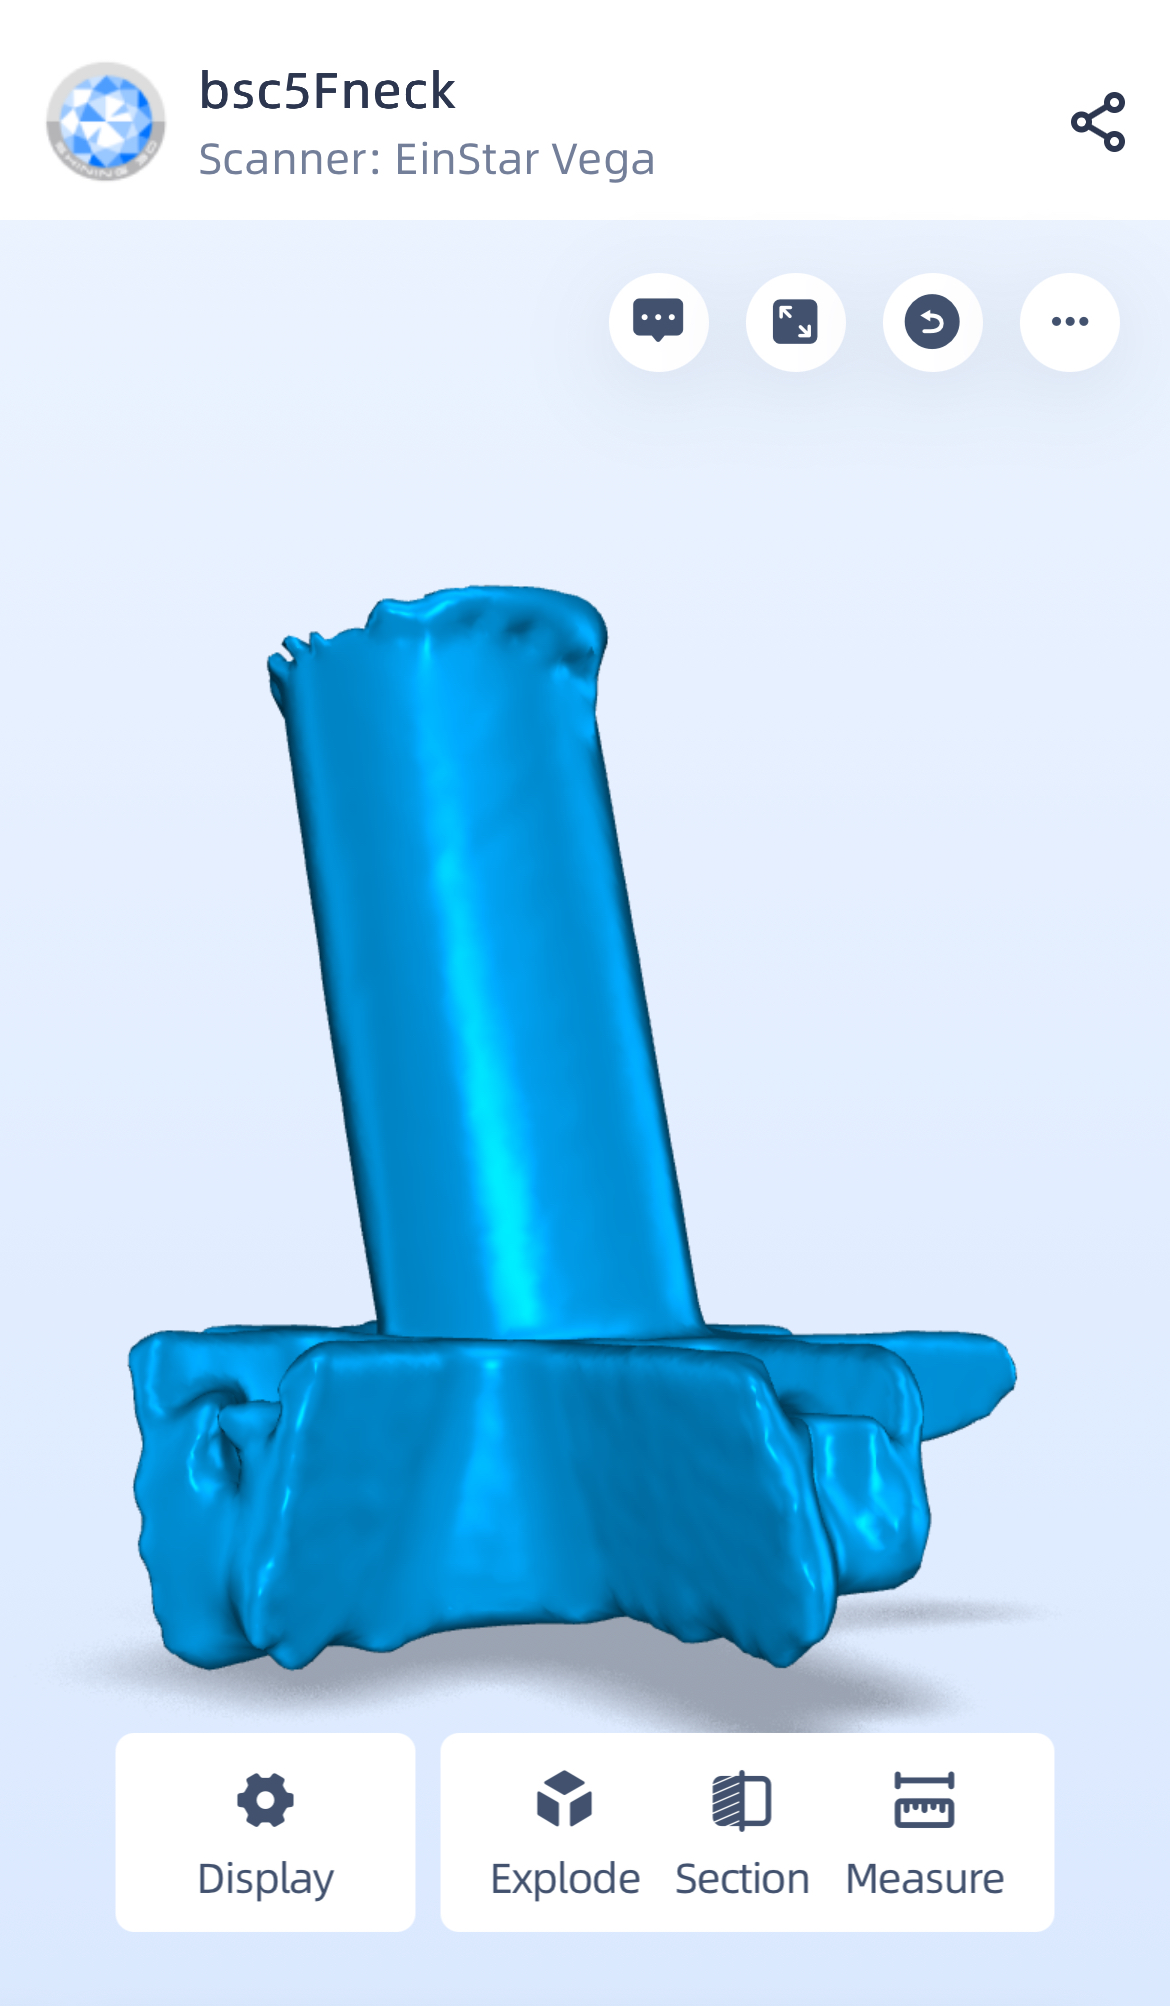
\includegraphics[width=0.9\textwidth]{media/scanned_roll.PNG}
    \caption{Unprocessed mesh of the paper roll as seen in the web viewer. The
      object contains artifacts such as the support (under the roll)
      and scanning
    inaccuracies (top of the roll).}
  \end{subfigure}
  ~
  \begin{subfigure}[t]{0.4\linewidth}
    \centering
    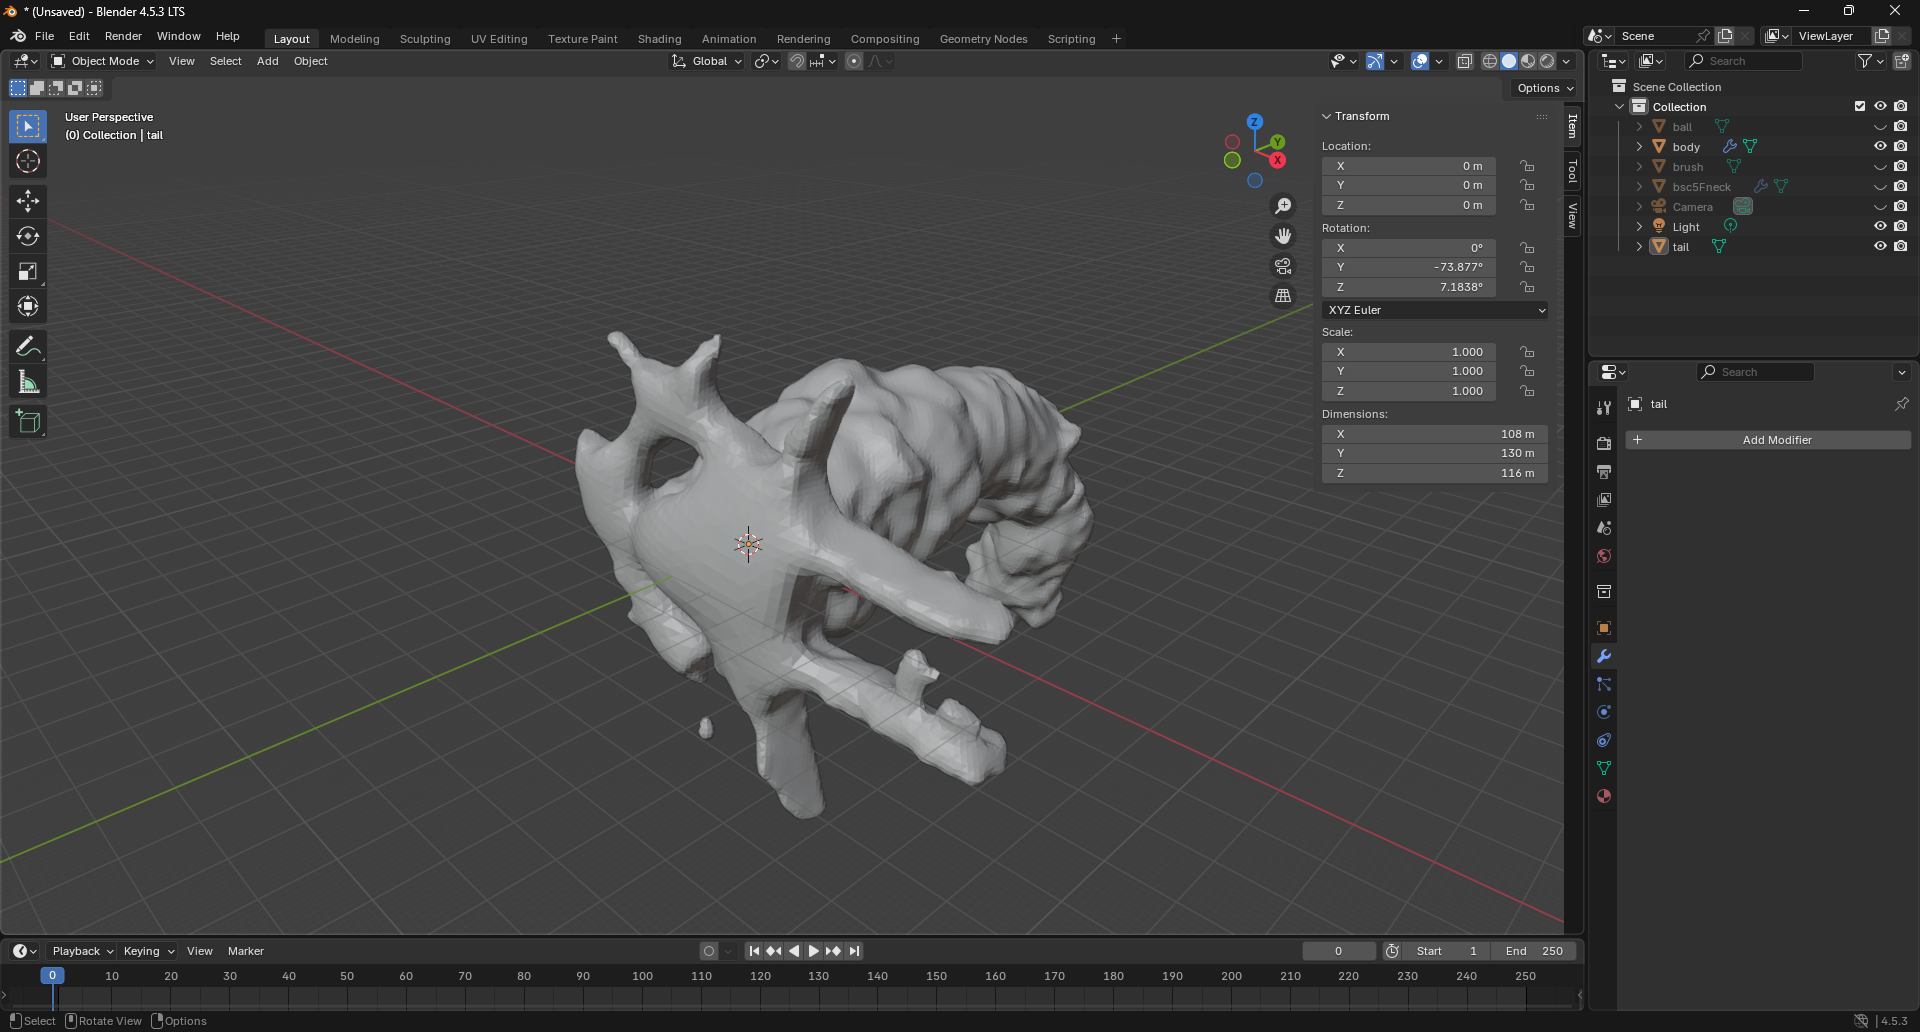
\includegraphics[width=0.9\textwidth]{media/blender_import.png}
    \caption{Imported object (dinglebop) in Blender.}
  \end{subfigure}
  ~
  \begin{subfigure}[t]{0.2\linewidth}
    \centering
    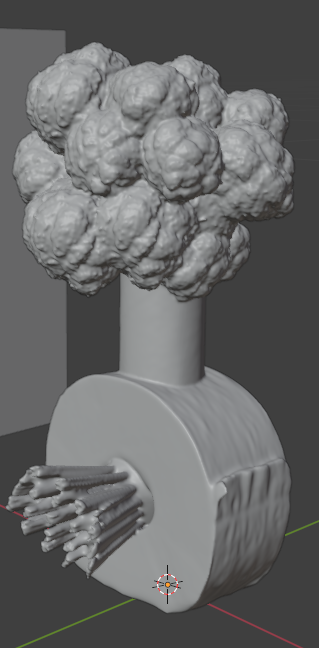
\includegraphics[width=0.9\textwidth]{media/blender_assembled.png}
    \caption{Assembled parts in Blender.}
  \end{subfigure}
  \caption{Steps of the scan cleanup process.}

\end{figure}

\section{3D Printing}

The second major milestone in the project timeline is the creation of a physical
object through 3D printing. To achieve this, the STL file was imported into
BambuStudio, the proprietary slicer made specifically for the hardware to be
used. The final orientation print setting were determined in the software.

Due to the complex shape of the plumbus, the amount and location of supports was
the guiding principle when placing the object on the build plate. Supports are
required when a section of the object cannot be supported by the object itself.
The most critical feature in the decision making was the chumbles, as removing
supports between the different pillars would have been difficult.
According to the previously mentioned considerations, through trial and error,
the most favorable orientation was found in which the least amount of support
material (waste) was used and the chumbles could be printed without the need of
support between each.

\end{document}
